%%% SIEDS 2026 submission. IEEEtran two-column conference template.

\documentclass[conference]{IEEEtran}
\IEEEoverridecommandlockouts

\usepackage{tabularx}
\usepackage{booktabs}
\usepackage{cite}
\usepackage{amsmath,amssymb,amsfonts}
\usepackage{algorithmic}
\usepackage{graphicx}
\usepackage{textcomp}
\usepackage{xcolor}
\usepackage{url}
\usepackage{array}

\graphicspath{{figures/}}

\def\BibTeX{{\rm B\kern-.05em{\sc i\kern-.025em b}\kern-.08em
    T\kern-.1667em\lower.7ex\hbox{E}\kern-.125emX}}

\begin{document}

\title{Optimising New York Citi Bike Station Occupancy:\\
A CTMC Model with Truck-Rebalancing-Rate Allocation}

\author{
\fontsize{10}{12}\selectfont
Spencer Arnold,
Paris Phan,
Garrett Uthlaut\\
\fontsize{9}{10}\selectfont \textit{School of Engineering and Applied Science, University of Virginia, Charlottesville, Virginia}
}

\maketitle

\begin{abstract}
New York City's Citi Bike system suffers from chronic spatial imbalance during commuter peaks: source stations near residential blocks run empty while destination stations near business districts overfill, and both failures force riders to abandon the system. We model each station as a finite-capacity continuous-time Markov chain (an M/M/1/K queue), extended with a Poisson truck-reset process that returns the station to a target fill level. Per-station failure rates are computed in closed form when no rebalancing is applied, or by direct linear solution of the stationary equation when rebalancing is added. For a five-station Midtown Manhattan cluster fit to December 2021 weekday morning trip data, we then solve the budget-constrained problem of allocating a total truck-visit-rate budget across the cluster to minimise long-run user failures, exactly via greedy marginal analysis on a discretised grid, exploiting the separable, convex-decreasing structure of the objective. At an operating budget of five truck-visits per hour across the cluster, the optimal allocation cuts long-run user failures from 41.87 to 1.77 events per hour, a 95.8 percent reduction; a Pareto-frontier sweep places the operational knee at 5.71 truck-visits per hour. We report sensitivity to ten percent rate perturbations and to the truck target-fill rule, and discuss validation alongside the limitations of the stationarity assumption.
\end{abstract}

\begin{IEEEkeywords}
bike-sharing, M/M/1/K queue, continuous-time Markov chain, rebalancing, marginal analysis, resource allocation
\end{IEEEkeywords}

\section{Introduction}

Citi Bike is the largest bike-sharing system in North America, operating roughly 25{,}000 bikes across more than 1{,}500 docking stations in Manhattan, Brooklyn, Queens, the Bronx, Jersey City and Hoboken \cite{citibike_data}. The system's core promise --- walk to a station, take a bike, ride to a destination, return the bike at the nearest station to where you are going --- breaks the moment a rider arrives at an empty source station or a saturated destination station. We refer to these two failure modes as \emph{stockout} (no bikes available for withdrawal) and \emph{dockblock} (no docks available for return); both convert a successful trip into a walk, a wait or an abandoned ride. During morning rush, directional commute flows produce predictable spatial imbalance: residential-area stations drain while business-district stations overfill.

The standard operational lever is \emph{truck rebalancing}: vehicles dispatched to redistribute bikes between stations. The rebalancing literature is sizeable \cite{schuijbroek2017,omahony2015,nair2013,lin2011}, but largely focuses on the vehicle-routing side --- which trucks visit which stations in what order. We pose a complementary question: given a total budget of truck-visit \emph{rates} across a station cluster, how should that budget be allocated across stations to minimise the long-run rate of user failures, and at what budget level does additional rebalancing stop paying for itself? The decision variable is the rate $\theta_n$ at which station $n$ is rebalanced --- a demand-side allocation question that is upstream of, and complementary to, the vehicle-routing problem.

Our contributions are: (i) a tractable continuous-time Markov chain (CTMC) model for a single Citi Bike station that augments the standard finite-capacity M/M/1/K queue \cite{gross2008,kleinrock1975} with an instantaneous Poisson truck-reset process; (ii) an exact greedy solver for the separable, integer-grid-discretised allocation problem $\min_{\theta} \sum_n F_n(\theta_n)$ subject to a budget constraint, justified by the strictly non-increasing marginal returns of $F_n$ in $\theta_n$; (iii) a Pareto frontier of cluster failure rate against budget, and a knee-detection result that locates the operational sweet spot \cite{satopaa2011}; and (iv) a sensitivity analysis quantifying how the optimum responds to $\pm 10\%$ perturbations in the empirical rate estimates and to the choice of truck target-fill rule.

We apply the framework to a five-station Midtown Manhattan cluster fitted to December 2021 trip data and find that an operating budget of five truck-visits per hour suffices to reduce cluster failures from 41.87 to 1.77 events per hour --- a 95.8\% reduction --- and that the Pareto knee at $\Theta = 5.71$ is within $1.1\times$ that operating point.

\section{System Model}\label{sec:model}

\subsection{Per-Station CTMC}

Consider a station $n$ with fixed dock capacity $c_n$. Let $s_n(t) \in \{0, 1, \ldots, c_n\}$ denote the number of bikes at the station at time $t$. We model two user-driven transitions and one operator-driven transition:

\begin{itemize}
\item \textbf{Withdrawal:} a rider arrives wanting a bike. Modelled as a Poisson process with rate $\lambda_n$ events per hour. Successful when $s_n > 0$ (transition $s_n \to s_n - 1$); a stockout event when $s_n = 0$.
\item \textbf{Deposit:} a rider arrives wanting to return a bike. Modelled as a Poisson process with rate $\mu_n$. Successful when $s_n < c_n$ (transition $s_n \to s_n + 1$); a dockblock when $s_n = c_n$.
\item \textbf{Truck reset:} a rebalancing visit arrives as a Poisson process with rate $\theta_n$. Each visit instantaneously resets the state to a target level $t_n$, where $t_n = \lfloor c_n / 2 \rfloor$ unless otherwise stated.
\end{itemize}

When $\theta_n = 0$, the resulting CTMC reduces to a finite-capacity birth-death chain that is structurally identical to the M/M/1/K queue with capacity $K = c_n$. Defining the dimensionless fill intensity $\rho_n = \mu_n / \lambda_n$, the stationary distribution has the standard closed form
\begin{equation}\label{eq:pi_closed}
\pi_k(n) = \frac{\rho_n^{\,k} (1 - \rho_n)}{1 - \rho_n^{\,c_n + 1}}, \qquad k = 0, 1, \ldots, c_n,
\end{equation}
with the limiting case $\pi_k = 1/(c_n + 1)$ when $\rho_n = 1$. We compute $\pi_k$ via a log-sum-exp normalisation to avoid overflow at the extreme values of $\rho$ that occur in practice (one cluster station has $\rho \approx 14$).

\subsection{Per-Station Failure Rate}

The long-run rate at which the station produces failed user events is
\begin{equation}\label{eq:Fn}
F_n = \lambda_n \, \pi_0(n) + \mu_n \, \pi_{c_n}(n),
\end{equation}
where the first term counts withdrawal attempts that arrive at an empty station (stockouts) and the second counts deposit attempts that arrive at a full station (dockblocks). $F_n$ depends on $(\lambda_n, \mu_n, c_n, \theta_n, t_n)$ through $\pi$.

\subsection{Truck-Reset Extension}

When $\theta_n > 0$, the multi-state jump $k \to t_n$ breaks the birth-death structure of the chain and the closed form (\ref{eq:pi_closed}) no longer applies. Instead we construct the $(c_n + 1) \times (c_n + 1)$ generator matrix $Q$:
\begin{align}
Q_{k,k+1} &= \mu_n \quad (0 \le k < c_n), \nonumber \\
Q_{k,k-1} &= \lambda_n \quad (0 < k \le c_n), \nonumber \\
Q_{k,t_n} &\mathrel{+}= \theta_n \quad (k \ne t_n), \label{eq:Q}\\
Q_{k,k} &= -\sum_{j \ne k} Q_{k,j}. \nonumber
\end{align}
The stationary distribution $\pi$ satisfies $\pi Q = 0$ with $\sum_k \pi_k = 1$ and is obtained as the unique probability vector solving this linear system (replacing the first row of $Q^\top$ with the normalisation constraint to eliminate the rank-one nullspace) using the SciPy dense LU solver \cite{virtanen2020}. Equation~(\ref{eq:Fn}) then gives $F_n(\theta_n)$.

The reduction to the closed form at $\theta_n = 0$ is exact and is verified numerically to floating-point precision (see Section~\ref{sec:validation}).

\section{Data and Cluster Selection}\label{sec:data}

\subsection{Trip and Station Data}

We use the public Citi Bike trip archive \cite{citibike_data} for December 2021, a representative pre-holiday month with a full set of weekday commuter mornings. Each row records the start station, end station, start and end timestamps, latitude--longitude pairs, and a member-vs-casual flag. The data was loaded with pandas, with timestamps cast and station identifiers reconciled against the General Bikeshare Feed Specification (GBFS) station feed \cite{gbfs} (which provides per-station capacities $c_n$). A total of 1{,}698{,}038 trip rows were ingested after dropping the small fraction with missing identifiers.

\subsection{Window and Rate Estimation}

We restrict to weekdays (Monday--Friday) in the window $[07{:}00, 10{:}00)$ local time --- the morning commute peak. December 2021 contains 23 weekdays in this window, giving an exposure of $69$ hours. For each station $n$ we estimate
\begin{equation}\label{eq:rate_estimation}
\hat\lambda_n = \frac{\#\{\text{trips with start at } n \text{ in window}\}}{\text{exposure hours}},
\end{equation}
and analogously for $\hat\mu_n$ on trip ends. We retain stations with $\ge 100$ events in the window and $\hat\lambda_n, \hat\mu_n > 0$, leaving 781 eligible stations. Using $\hat\rho_n = \hat\mu_n / \hat\lambda_n$, we classify each station as \emph{source} ($\rho < 0.7$, $n = 291$), \emph{balanced} ($0.7 \le \rho \le 1.5$, $n = 343$), or \emph{sink} ($\rho > 1.5$, $n = 147$).

\subsection{Cluster Selection}

To exhibit the full source--sink interaction that rebalancing acts on, we score candidate clusters by
\[
\text{score} = (\text{total events}) \times \min(V_s, V_d) / \max(V_s, V_d) \times \overline{|\log \rho|},
\]
where $V_s, V_d$ are the source and sink event volumes in the cluster. The factor $\min/\max$ explicitly penalises monocultures of sources or sinks. Seeds are top-volume sinks; each seed is expanded with the top three origin stations by trip count and an optional nearby secondary sink within 1\,km (haversine). The hard gates are: at least one source, at least one sink, and at least 2{,}000 events in the window.

The top-scoring cluster has five members in Midtown Manhattan (\(W\,31\)--\(58\) St, \(5\)--\(11\) Ave, with one Madison Ave station). Cluster characteristics are reported in Table~\ref{tab:cluster}. The cluster aggregates 8{,}093 events in the window, has total capacity $\sum c_n = 349$ docks, and a balance factor of $0.913$. Notably, only 2.4\% of deposits into the cluster's sinks originate at cluster sources --- the cluster is mostly fed by exogenous origins, which has implications we return to in Section~\ref{sec:validation}.

\begin{table}[t]
\caption{Selected five-station Midtown cluster (Dec 2021, 07{:}00--10{:}00 weekdays).}
\label{tab:cluster}
\centering
\renewcommand{\arraystretch}{1.1}
\setlength{\tabcolsep}{4pt}
\begin{tabular}{@{}lccccc@{}}
\toprule
Station & Type & $\hat\lambda$ & $\hat\mu$ & $\hat\rho$ & $c$ \\
& & (/h) & (/h) & & (docks) \\
\midrule
Madison Ave \& E\,51 St & sink     & 1.25  & 17.90 & 14.36 & 43 \\
W\,42 St \& 6 Ave        & balanced & 8.87  & 13.00 & 1.47  & 53 \\
8 Ave \& W\,31 St        & source   & 23.64 & 11.01 & 0.47  & 97 \\
Broadway \& W\,58 St     & balanced & 11.65 & 11.14 & 0.96  & 79 \\
W\,55 St \& 6 Ave        & sink     & 5.45  & 13.38 & 2.45  & 77 \\
\bottomrule
\end{tabular}
\end{table}

A goodness-of-fit check on the inter-arrival distributions shows that the Poisson assumption is rejected on most cluster streams; we present the assumption as a model choice and defer the diagnostic table to Section~\ref{sec:validation}.

\section{Optimisation Method}\label{sec:opt}

\subsection{From Capacity Reallocation to Rebalancing-Rate Allocation}

The original problem framing posed a fixed-capacity reallocation question: with $\sum c_n$ held constant, search for the integer allocation $(c_1^*, \ldots, c_N^*)$ that minimises the cluster failure rate. For our cluster this lever is empirically inert. Three of the five stations have $\rho \in \{0.47, 2.45, 14.36\}$ --- all in the asymptotic regime of (\ref{eq:pi_closed}), where $\pi_0$ or $\pi_{c_n}$ is already saturated within numerical precision. Adding or removing one dock changes $F_n$ by less than $10^{-10}$, so any plausible reallocation moves the cluster total by an unobservable amount. We therefore switch the lever to the rebalancing rate $\theta_n$, which directly attacks the boundary probabilities through the truck-reset transition in (\ref{eq:Q}).

\subsection{Problem Statement}

Given a total rebalancing budget $\Theta_{\text{total}}$ (in truck-visits per hour aggregated across the cluster), allocate it across the $N = 5$ stations to minimise long-run cluster failure:
\begin{equation}\label{eq:opt}
\begin{aligned}
\min_{\theta_1, \ldots, \theta_N \ge 0} \quad & F(\theta_1, \ldots, \theta_N) = \sum_{n=1}^{N} F_n(\theta_n) \\
\text{subject to} \quad & \sum_{n=1}^{N} \theta_n = \Theta_{\text{total}}.
\end{aligned}
\end{equation}
The objective is separable in $\theta_n$, and each $F_n$ is monotone non-increasing and convex in $\theta_n$ (verified numerically across the relevant range; see Section~\ref{sec:results}).

\subsection{Greedy Marginal Analysis}

Discretise the budget into steps of $\delta = 0.01$. Initialise $\theta_n^{(0)} = 0$ for all $n$. At iteration $k$, allocate one increment $\delta$ to the station with the largest marginal failure reduction:
\begin{equation}\label{eq:greedy}
n^{(k)} = \arg\max_n \left[ F_n(\theta_n^{(k-1)}) - F_n(\theta_n^{(k-1)} + \delta) \right],
\end{equation}
update $\theta_{n^{(k)}}^{(k)} \leftarrow \theta_{n^{(k)}}^{(k-1)} + \delta$, and continue until the cumulative budget reaches $\Theta_{\text{total}}$. Because the per-station marginal reduction is strictly non-increasing in $\theta_n$ (each $F_n$ is convex), the greedy procedure is provably optimal for the discretised problem and produces, by construction, the same total at $\Theta_{\text{total}}$ as any exact integer-grid optimiser. We verify the non-increasing-returns property at every step of every run (zero violations across all reported experiments).

\subsection{Pareto Frontier via Nested Prefix}

A useful structural property of greedy is that the allocation at any budget $B' \le B$ is exactly the prefix of the allocation produced at budget $B$ truncated at $B'$. We therefore execute the greedy once at $\max(\Theta_{\text{total}})$, save the per-step trajectory, and sample it at any required budget. This yields the full Pareto frontier $F^*(\Theta_{\text{total}})$ in a single greedy pass.

We locate the operational knee of the frontier using the kneedle method \cite{satopaa2011}: normalise both axes to $[0, 1]$, draw the chord from the unconstrained endpoint to the saturated endpoint, and report the budget at which the curve falls farthest below the chord.

\section{Results}\label{sec:results}

\subsection{Base Model}

With all rates and capacities held at their estimated values and $\theta_n = 0$, the cluster's per-station failure rates and stockout/dockblock decomposition are reported in Table~\ref{tab:base}. The cluster aggregate is
\[
F_{\text{base}} = \sum_n F_n(0) = 41.87 \text{ events / hour},
\]
which corresponds to about 126 failed user events per three-hour weekday morning. The composition is essentially balanced, with stockouts (12.62/h, all from 8\,Ave \& W\,31 St) almost matching dockblocks (29.25/h, dominated by Madison\,Ave\,\&\,E\,51 St at 16.65/h and W\,55 St \& 6 Ave at 7.93/h).

\begin{table}[t]
\caption{Base-model per-station results at $\theta = 0$.}
\label{tab:base}
\centering
\renewcommand{\arraystretch}{1.1}
\setlength{\tabcolsep}{3pt}
\begin{tabular}{@{}lccccc@{}}
\toprule
Station & $\pi_0$ & $\pi_c$ & $F_n$ & stockout & dockblock \\
& & & (/h) & (/h) & (/h) \\
\midrule
Madison \& E\,51 St   & $\sim\!10^{-50}$ & 0.930 & 16.65 & 0.00  & 16.65 \\
W\,42 St \& 6 Ave      & $\sim\!10^{-9}$  & 0.318 & 4.13  & 0.00  & 4.13  \\
8 Ave \& W\,31 St      & 0.534            & $\sim\!10^{-32}$ & 12.62 & 12.62 & 0.00  \\
Broadway \& W\,58 St   & 0.045            & 0.001 & 0.54  & 0.52  & 0.01  \\
W\,55 St \& 6 Ave      & $\sim\!10^{-31}$ & 0.593 & 7.93  & 0.00  & 7.93  \\
\midrule
\textbf{Total}         &                  &       & \textbf{41.87} & \textbf{13.15} & \textbf{28.72} \\
\bottomrule
\end{tabular}
\end{table}

\subsection{Per-Station Response Curves}

Sweeping $\theta_n$ over a log-spaced grid from $0.1$ to $10$ events/hour, we trace each $F_n(\theta_n)$ in Figure~\ref{fig:response}. All five curves are monotone non-increasing, smooth, and visually convex, confirming the property that justifies the greedy solver. The two extreme stations --- Madison \& E\,51 St ($\rho = 14.4$, sink) and 8\,Ave \& W\,31 St ($\rho = 0.47$, source) --- carry the most reducible failure mass. The right-hand panel shows the underlying mechanism: $\pi_0$ for the source and $\pi_c$ for the heaviest sinks fall by orders of magnitude as $\theta$ grows, while the boundary probabilities of the already-balanced stations are essentially zero from the start.

\begin{figure*}[t]
\centering
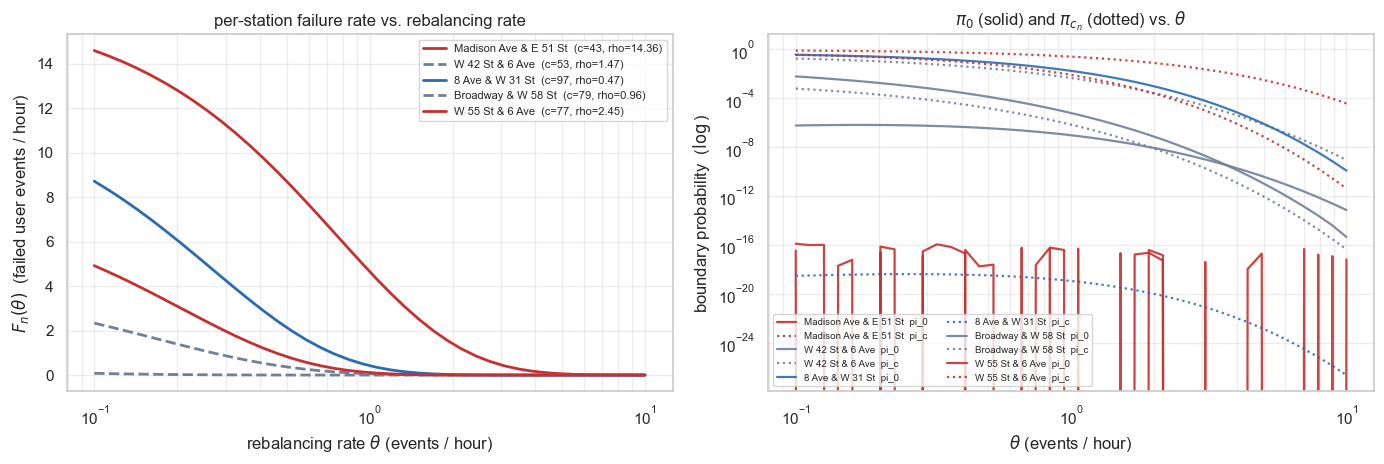
\includegraphics[width=\textwidth]{fig_response_curves.png}
\caption{Per-station response to rebalancing rate $\theta$. \textbf{Left:} long-run failure rate $F_n(\theta)$ for each cluster station, log-$x$. The two extremes (Madison \& E\,51, 8 Ave \& W\,31) carry the largest reducible failure mass; the near-balanced station (Broadway \& W\,58) starts close to zero. \textbf{Right:} stationary boundary probabilities $\pi_0$ (solid) and $\pi_{c_n}$ (dotted), log-$y$, showing the mechanism by which $\theta$ reduces each station's dominant failure mode.}
\label{fig:response}
\end{figure*}

\subsection{Single-Budget Optimisation}

We pick an operating budget of $\Theta_{\text{total}} = 5$ events/hour, which corresponds operationally to ``approximately one truck-visit per station per hour on average'' across the cluster. Running greedy at this budget yields the per-station allocations and outcomes in Table~\ref{tab:opt}.

\begin{table}[t]
\caption{Optimal allocation at $\Theta_{\text{total}} = 5$ events/h.}
\label{tab:opt}
\centering
\renewcommand{\arraystretch}{1.1}
\setlength{\tabcolsep}{3pt}
\begin{tabular}{@{}lcccc@{}}
\toprule
Station & $\theta_n^*$ & $F_n^{\text{base}}$ & $F_n^{\text{opt}}$ & $\Delta$ \\
& (/h) & (/h) & (/h) & \\
\midrule
Madison \& E\,51 St   & 2.42 & 16.65 & 0.87 & $-94.8\%$ \\
W\,42 St \& 6 Ave      & 0.59 & 4.13  & 0.26 & $-93.8\%$ \\
8 Ave \& W\,31 St      & 1.09 & 12.62 & 0.32 & $-97.5\%$ \\
Broadway \& W\,58 St   & 0.11 & 0.54  & 0.07 & $-87.1\%$ \\
W\,55 St \& 6 Ave      & 0.79 & 7.93  & 0.25 & $-96.8\%$ \\
\midrule
\textbf{Cluster}       & \textbf{5.00} & \textbf{41.87} & \textbf{1.77} & $\boldsymbol{-95.8\%}$ \\
\bottomrule
\end{tabular}
\end{table}

The cluster failure rate falls from $F_{\text{base}} = 41.87$ to $F_{\text{opt}} = 1.77$ events per hour, a $95.8\%$ reduction. Roughly half the budget is allocated to the most extreme sink (Madison \& E\,51, $\theta^* = 2.42$, $\rho = 14.4$); the remainder concentrates on the extreme source (8 Ave \& W\,31, $\theta^* = 1.09$). The near-balanced station Broadway \& W\,58 ($\rho = 0.96$, $F_n^{\text{base}} = 0.54$) receives only $\theta^* = 0.11$: greedy correctly recognises that rebalancing a station whose failure rate is already small is poor return on budget. Figure~\ref{fig:bars} visualises the before/after per-station bars.

\begin{figure}[t]
\centering
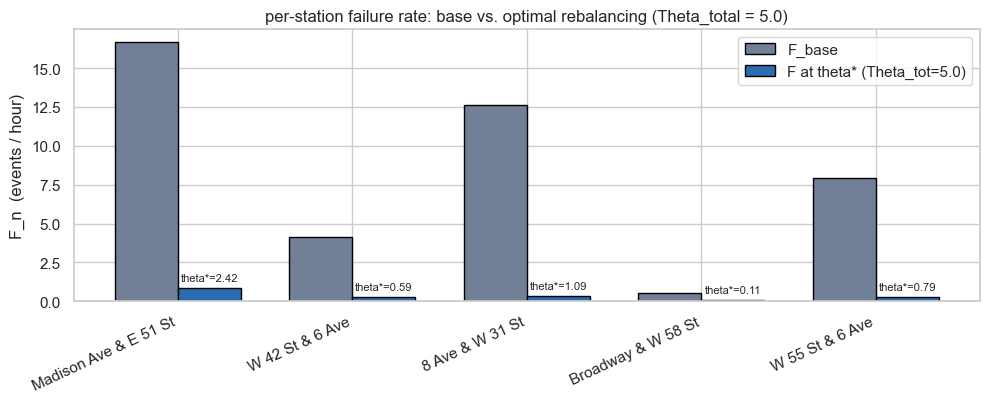
\includegraphics[width=\columnwidth]{fig_base_vs_opt.png}
\caption{Per-station failure rate before (grey) and after (blue) optimal rebalancing at $\Theta_{\text{total}} = 5$, with the assigned $\theta_n^*$ annotated.}
\label{fig:bars}
\end{figure}

\subsection{Pareto Frontier and Knee}

Sweeping $\Theta_{\text{total}} \in [0, 50]$ via the nested-prefix construction yields the Pareto frontier in Figure~\ref{fig:pareto}, left panel. The frontier is steep up to $\Theta \approx 6$ and then flattens to near zero. The kneedle detector locates the operational knee at
\[
\Theta_{\text{knee}} = 5.71 \text{ events/hour}, \quad F_{\text{knee}} = 1.20 \text{ (}{-97.1\%}\text{)},
\]
which is within $1.14\times$ of our chosen operating budget, confirming that $\Theta = 5$ sits on the steep, high-marginal-return part of the curve. Beyond the knee the frontier is essentially flat and additional rebalancing buys negligible improvement; below it, marginal returns are large and any reduction in the budget is costly. The right panel of Figure~\ref{fig:pareto} shows that as the budget grows, allocation goes first to the heaviest sink, then to the heaviest source, with the near-balanced stations always trailing.

\begin{figure*}[t]
\centering
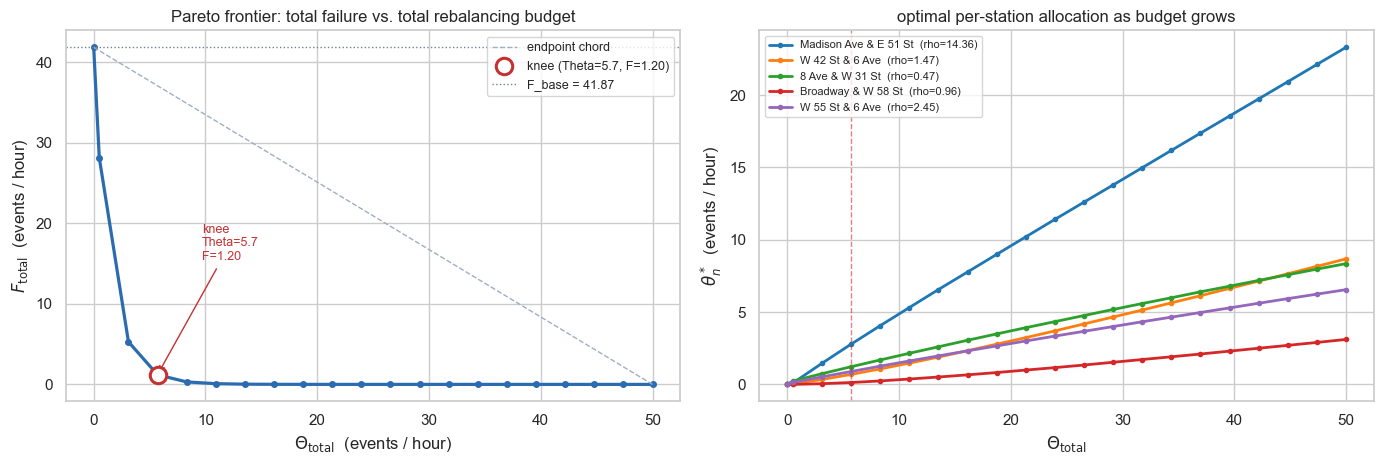
\includegraphics[width=\textwidth]{fig_pareto.png}
\caption{\textbf{Left:} Pareto frontier of cluster failure rate vs.\ total rebalancing budget. The knee at $\Theta = 5.71$ (red circle) marks the transition from steep to saturated marginal returns. The endpoint chord (dashed grey) is the kneedle-method baseline. \textbf{Right:} per-station optimal allocation $\theta_n^*$ as a function of $\Theta_{\text{total}}$. Madison \& E\,51 (heaviest sink) absorbs the largest share at every budget; Broadway \& W\,58 (near-balanced) tracks near zero.}
\label{fig:pareto}
\end{figure*}

\section{Sensitivity Analysis}\label{sec:sensitivity}

\subsection{Rate Perturbations}

To assess the impact of rate-estimation error, we perturb each of $\hat\lambda_n$ and $\hat\mu_n$ by $\pm 10\%$ one at a time and re-solve at $\Theta_{\text{total}} = 5$ (twenty perturbation runs). The largest absolute swing in $F_{\text{opt}}$ is $\pm 0.37$ events/hour --- about $\pm 21\%$ relative to the unperturbed $F_{\text{opt}} = 1.77$, but only $\pm 0.9\%$ relative to the unperturbed $F_{\text{base}} = 41.87$. The largest $L_1$ shift in the allocation vector $\theta^*$ is $0.32$ out of a budget of $5.00$, i.e.\ $6.4\%$ of the total. The post-optimisation \emph{number} is sensitive to the rate estimates; the post-optimisation \emph{policy} much less so.

\subsection{Truck Target-Fill Rule}

The default target $t_n = \lfloor c_n / 2 \rfloor$ (``half-full after a truck visit'') is a modelling assumption rather than something estimated from data. We re-solve at $\Theta = 5$ under three target rules:
\begin{center}
\begin{tabular}{@{}lcc@{}}
\toprule
Target rule & $F_{\text{opt}}$ (/h) & $\Delta$ vs.\ $c/2$ \\
\midrule
$t_n = \lfloor c_n / 3 \rfloor$  & 1.41 & $-0.36$ \\
$t_n = \lfloor c_n / 2 \rfloor$  & 1.77 & --- \\
$t_n = \lfloor 2 c_n / 3 \rfloor$ & 3.58 & $+1.82$ \\
\bottomrule
\end{tabular}
\end{center}

The 2/3-full target roughly doubles $F_{\text{opt}}$ relative to half-full --- the target rule is the most load-bearing modelling assumption in the analysis. We retain $\lfloor c_n/2 \rfloor$ as the operationally defensible default: it symmetrically defends against both stockout and dockblock, and matches the implicit goal of dispatch crews who balance between empty and full.

\section{Validation and Limitations}\label{sec:validation}

\subsection{Numerical Validation of the Model and Solver}

Two non-trivial properties were verified by automated tests run after every code change:
\begin{enumerate}
\item At $\theta_n = 0$, the linear-system solution $\pi$ from solving $\pi Q = 0$ coincides with the closed-form geometric distribution (\ref{eq:pi_closed}) to absolute tolerance $10^{-10}$ on every test case. This guarantees that the rebalancing extension is a strict generalisation of the M/M/1/K base model with no spurious deviation at the boundary $\theta = 0$.
\item The marginal reduction $F_n(\theta_n) - F_n(\theta_n + \delta)$ is non-increasing in $\theta_n$ at every step of every greedy run reported in this paper. Zero monotonicity violations were observed across the single-budget run, the 21-point Pareto sweep, the 20-point rate-perturbation set, and the three-point target-rule sweep --- confirming that the greedy solution is exact, not approximate.
\end{enumerate}

\subsection{Inter-Arrival Goodness of Fit}

The model treats withdrawals and deposits as Poisson processes, equivalent to assuming exponential inter-arrival times within the morning window. We test this directly with a chi-squared and Kolmogorov--Smirnov goodness-of-fit on same-day inter-arrival samples (cross-day gaps excluded since the rate process resets nightly). Table~\ref{tab:gof} summarises the results.

\begin{table}[t]
\caption{Exponential goodness-of-fit on same-day inter-arrivals. Pass requires both chi-squared $p > 0.05$ and KS $p > 0.05$.}
\label{tab:gof}
\centering
\renewcommand{\arraystretch}{1.05}
\setlength{\tabcolsep}{3pt}
\begin{tabular}{@{}llcccc@{}}
\toprule
Station & Event & $n$ & $\chi^2 \, p$ & KS $p$ & Pass \\
\midrule
Madison \& E\,51 & withdraw & 64   & 0.185 & 0.462 & \checkmark \\
Madison \& E\,51 & deposit  & 1212 & 0.000 & 0.000 & --- \\
W\,42 \& 6 Ave    & withdraw & 590  & 0.000 & 0.000 & --- \\
W\,42 \& 6 Ave    & deposit  & 875  & 0.000 & 0.000 & --- \\
8 Ave \& W\,31    & withdraw & 1608 & 0.000 & 0.000 & --- \\
8 Ave \& W\,31    & deposit  & 737  & 0.115 & 0.048 & --- \\
Broadway \& W\,58 & withdraw & 785  & 0.002 & 0.001 & --- \\
Broadway \& W\,58 & deposit  & 750  & 0.007 & 0.000 & --- \\
W\,55 \& 6 Ave    & withdraw & 354  & 0.022 & 0.039 & --- \\
W\,55 \& 6 Ave    & deposit  & 900  & 0.025 & 0.000 & --- \\
\bottomrule
\end{tabular}
\end{table}

Nine of the ten streams reject the exponential at the joint $p > 0.05$ threshold. This is consistent with genuine non-stationarity within the three-hour window: the morning-rush rate ramps up from 7\,AM, peaks around 8\,AM, and tails off by 9{:}30. Fitting a constant rate to a non-stationary process inflates the within-window variance of inter-arrivals beyond what an exponential allows. We do \emph{not} attempt to ``rescue'' the fit by narrowing the window or by selecting a less imbalanced cluster; instead we present the CTMC as a model under the constant-rate assumption and treat the GOF rejection as a known modelling limitation. The optimisation results in Sections~\ref{sec:results}--\ref{sec:sensitivity} should be read as the optimum of the model, not as ground truth for the underlying system. Figure~\ref{fig:qq} shows the corresponding Q-Q diagnostic and inter-arrival histograms.

\begin{figure}[t]
\centering
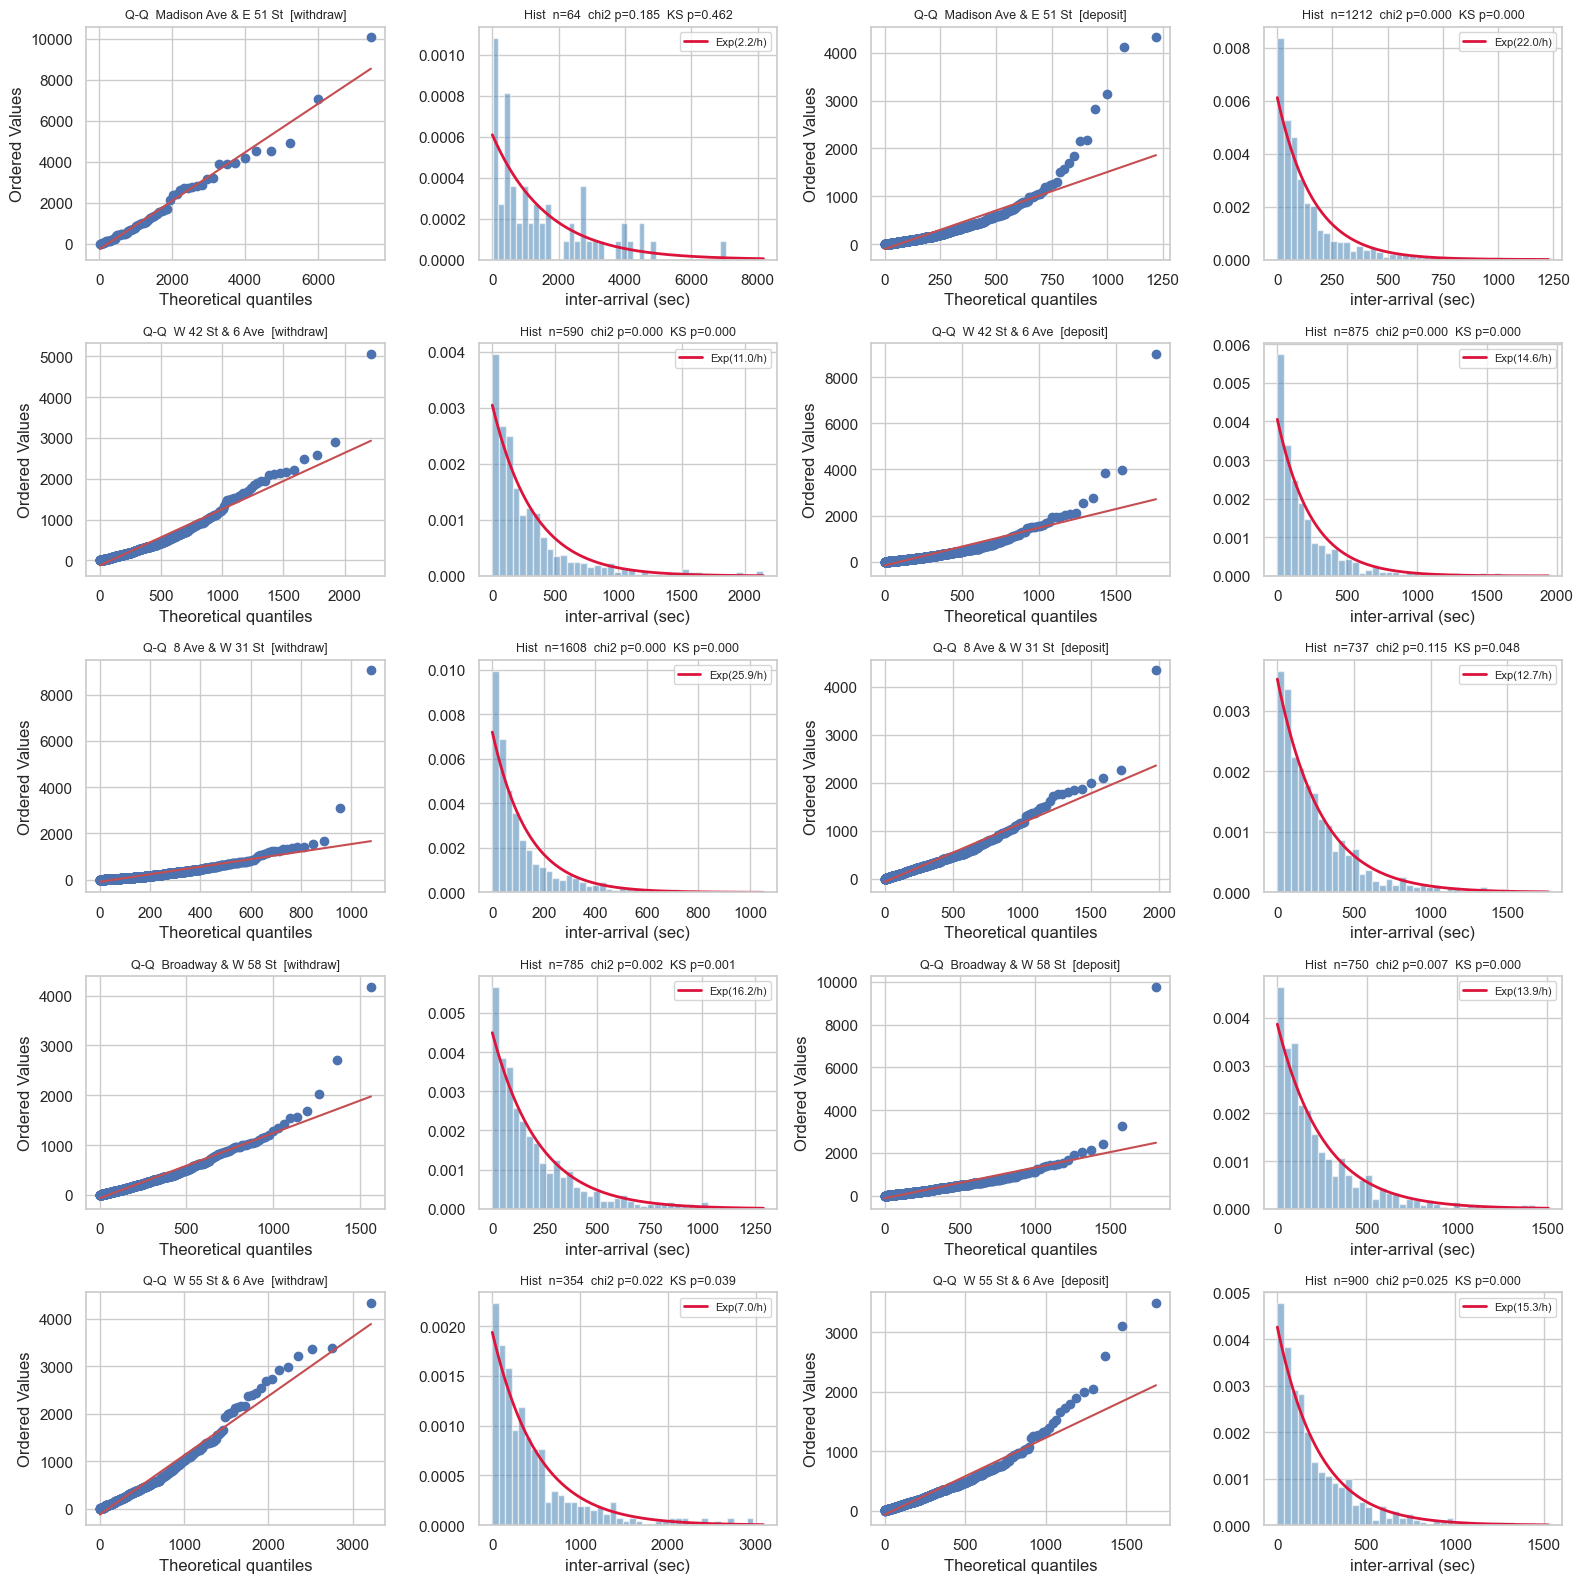
\includegraphics[width=\columnwidth]{fig_qq.png}
\caption{Exponential goodness-of-fit diagnostics for each (station, event-type) inter-arrival stream: Q-Q plot (left of each pair) and histogram with fitted exponential PDF (right). Departures from the diagonal in the Q-Q plots are concentrated in the upper tail, consistent with within-window rate non-stationarity.}
\label{fig:qq}
\end{figure}

\subsection{Other Limitations}

\textbf{Closure fraction.} The five-station cluster receives only about 2.4\% of its sink-bound deposits from cluster sources. The independent-station CTMC is reasonable here precisely because most arrivals are exogenous --- but it also means that the optimal $\theta^*$ vector is implicitly conditioned on those exogenous flows holding constant. A larger-scale rollout that perturbs many stations simultaneously would need a network model that propagates the second-order effects.

\textbf{Capacity drift.} The GBFS feed reports present-day capacities; some stations may have been reconfigured since December 2021. The base-model $\pi$ is most sensitive to $c_n$ for near-balanced stations, but our two near-balanced cluster members (Broadway \& W\,58, W\,42 \& 6 Ave) carry small absolute failure mass, so the sensitivity is bounded.

\textbf{No balking model.} Users who encounter a stockout or dockblock are assumed to exit the system rather than walking to a neighbouring station. Balking would couple the per-station chains and is left to future work.

\textbf{Demand-side optimisation only.} We optimise the allocation of rebalancing-visit \emph{rates}, not the routing of the trucks that deliver them. The question of whether a fleet can physically realise a given $(\theta_1, \ldots, \theta_N)$ is a vehicle-routing problem that complements --- but is distinct from --- the allocation problem solved here.

\section{Conclusion and Future Work}

We modelled a five-station Citi Bike cluster as independent finite-capacity Markov chains with Poisson truck-reset transitions and showed that an exact greedy marginal-analysis solver reduces cluster-wide morning-rush user failures by $95.8\%$ at an operating budget of five truck-visits per hour, with the Pareto knee at $\Theta = 5.71$ giving a near-identical $97.1\%$ reduction. The optimal allocation is concentrated on the cluster's two extremes: the heaviest sink and the heaviest source absorb 70\% of the budget. Sensitivity is moderate to rate-estimation error and meaningful but bounded under reasonable variations of the truck target-fill rule.

Several extensions are natural. First, the current single-station model could be replaced with a closed-loop network simulation that propagates rebalancing across the system and captures the second-order coupling that the independence assumption suppresses. Second, a time-varying $\lambda(t), \mu(t)$ within the morning window would directly address the non-stationarity that drove the GOF rejections, at the cost of losing the closed-form stationary distribution. Third, a complementary user-incentive lever --- dynamic pricing that discounts deposits at empty stations and surcharges deposits at full ones --- could turn riders into a self-rebalancing force, complementing the truck-rate allocation studied here. Fourth, the rate allocations $(\theta_1, \ldots, \theta_N)$ produced by the model serve as an upstream input to a downstream vehicle-routing optimisation: how can a fixed truck fleet realise the prescribed allocation while respecting routing constraints?

\section*{Acknowledgment}

The authors thank the SYS 3060 teaching staff at the University of Virginia for guidance on model validation, and Citi Bike NYC for releasing the trip-history data that made this work possible.

\begin{thebibliography}{00}

\bibitem{citibike_data} Lyft, Inc., ``Citi Bike system data,'' 2024. [Online]. Available: \url{https://citibikenyc.com/system-data}.

\bibitem{gbfs} MobilityData, ``General Bikeshare Feed Specification (GBFS),'' v3.0, 2023. [Online]. Available: \url{https://github.com/MobilityData/gbfs}.

\bibitem{gross2008} D. Gross, J. F. Shortle, J. M. Thompson, and C. M. Harris, \emph{Fundamentals of Queueing Theory}, 4th ed. Hoboken, NJ: Wiley, 2008.

\bibitem{kleinrock1975} L. Kleinrock, \emph{Queueing Systems, Volume 1: Theory}. New York, NY: Wiley, 1975.

\bibitem{schuijbroek2017} J. Schuijbroek, R. C. Hampshire, and W.-J. van Hoeve, ``Inventory rebalancing and vehicle routing in bike sharing systems,'' \emph{European Journal of Operational Research}, vol.~257, no.~3, pp.~992--1004, 2017.

\bibitem{omahony2015} E. O'Mahony and D. B. Shmoys, ``Data analysis and optimization for (Citi)Bike sharing,'' in \emph{Proc.\ AAAI Conf.\ Artificial Intelligence}, vol.~29, no.~1, 2015, pp.~687--694.

\bibitem{nair2013} R. Nair, E. Miller-Hooks, R. C. Hampshire, and A. Bu\v{s}i\'c, ``Large-scale vehicle sharing systems: Analysis of V\'elib','' \emph{International Journal of Sustainable Transportation}, vol.~7, no.~1, pp.~85--106, 2013.

\bibitem{lin2011} J.-R. Lin and T.-H. Yang, ``Strategic design of public bicycle sharing systems with service level constraints,'' \emph{Transportation Research Part E: Logistics and Transportation Review}, vol.~47, no.~2, pp.~284--294, 2011.

\bibitem{satopaa2011} V. Satop\"a\"a, J. Albrecht, D. Irwin, and B. Raghavan, ``Finding a `kneedle' in a haystack: Detecting knee points in system behavior,'' in \emph{Proc.\ 31st International Conference on Distributed Computing Systems Workshops}, 2011, pp.~166--171.

\bibitem{virtanen2020} P. Virtanen \emph{et al.}, ``SciPy 1.0: Fundamental algorithms for scientific computing in Python,'' \emph{Nature Methods}, vol.~17, pp.~261--272, 2020.

\end{thebibliography}

\end{document}
